\documentclass{beamer}
\usepackage{tikz}
\usetikzlibrary{positioning, backgrounds, fit}

\newcommand{\indep}{\raisebox{0.05em}{\rotatebox[origin=c]{90}{$\models$}}}
\newcommand{\nindep}{{\rotatebox[origin=c]{90}{$\nvDash$}}}

\usetheme{default}

\title{Estimating bayesian graphical models with EM}
\author{Luca Bracone}
\begin{document}
\begin{frame}{Undirected bayesian graph}
	\begin{center}
		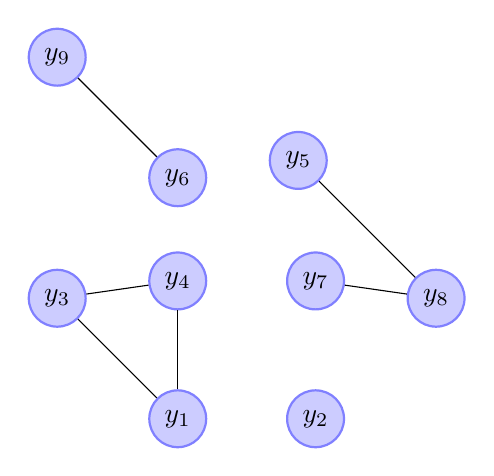
\begin{tikzpicture}
			[gene/.style={circle, draw=blue!50, fill=blue!20, thick }]
			\node[gene] (g1) [] {$y_1$};
			\node[gene] (g2) [right = of g1] {$y_2$};
			\node[gene] (g3) [above left = of g1] {$y_3$}
			edge (g1)
			;
			\node[gene] (g4) [above = of g1] {$y_4$}
			edge (g3)
			edge (g1)
			;
			\node[gene] (g5) [above right = of g4] {$y_5$};
			\node[gene] (g6) [above right = of g3] {$y_6$};
			\node[gene] (g7) [above  = of g2] {$y_7$};
			\node[gene] (g8) [above right = of g2] {$y_8$}
			edge node{} (g7)
			edge node{} (g5);
			\node[gene] (g9) [above left = of g6] {$y_9$}
			edge node{} (g6);
		\end{tikzpicture}
	\end{center}
	There is an edge $(i,j)$ if and only if $y_i \nindep y_j | y_{-ij}$
\end{frame}
\begin{frame}{Setting and assumptions}
	We observe $p$ gene expression levels across $n$ patients. That is we have
	$n$ observations $y_1, \dots, y_n \in \mathbb{R}^p$ of a $p$ dimensional
	vector. We assume that $y_1, \dots, y_n \stackrel{i.i.d.}{\sim}
		\mathcal{N}_p(0, \Sigma)$ have a multivariate normal distribution.
	\begin{itemize}
		\item To estimate the graph we would like to know whether $y_i \nindep
			      y_j | y_{-ij}$.
		\item Idea: We know that in the \emph{precision matrix,} $\Omega =
			      \Sigma^{-1}$ the $(i,j)$-th entry is zero only if $y_i \indep y_j |
			      y_{-ij}$
		\item How do we find the zero entries of $\Omega$ ?
	\end{itemize}
\end{frame}
\begin{frame}{Why should we use the Bayesian method ?}
	\begin{itemize}
		\item We have access to the empirical precision matrix, we could derive
		      statistical tests.
		\item This method becomes cumbersome when the number of parameters $p$
		      becomes large.
	\end{itemize}
	If we consider $\Omega$ as being drawn from a prior distribution
	$p(\Omega)$ we can obtain a \emph{posterior distrbution} $p(\Omega | X)$
	of which the maximum is the \emph{maximum à-posteriori} estimate
	$\Omega$.
\end{frame}
\begin{frame}{Spike and slab prior}
	The spike and slab prior for $\Omega$ helps us differentiate between zero
	and non-zero entries of $\Omega$
	\begin{align*}
		y | \Omega                & \sim N_p(0, \Omega^{-1}),                                                          \\
		\omega_{ij} | \delta_{ij} & \sim \delta_{ij} N(0, v_1^2) + (1 - \delta_{ij}) N(0, v_0^2) \text{for } i \neq j, \\
		\omega_{ii}               & \sim Exp(\lambda/2),                                                               \\
		\delta_{ij} | \pi         & \sim Bern(\pi),                                                                    \\
		\pi                       & \sim Beta(a,b).
	\end{align*}
	After a few manipulations we find that
	\[ p(\Omega, \delta, \pi | y) \propto p(y | \Omega) p(\Omega | \delta) p(\delta | \pi) p(\pi) \]
\end{frame}
\begin{frame}
	k
\end{frame}
\end{document}
